%% ---------------------------------------------------------------
%% Background
%% (C) AmirHossein Sojoodi @ Queen's University - 2020
%% ---------------------------------------------------------------

\chapter{Background}
\label{ch-background}

\lipsum[1-1]
This is a reference to a dummy diagram: \ref{fig:Dummy-Figure}.

\begin{figure}
	\centering
	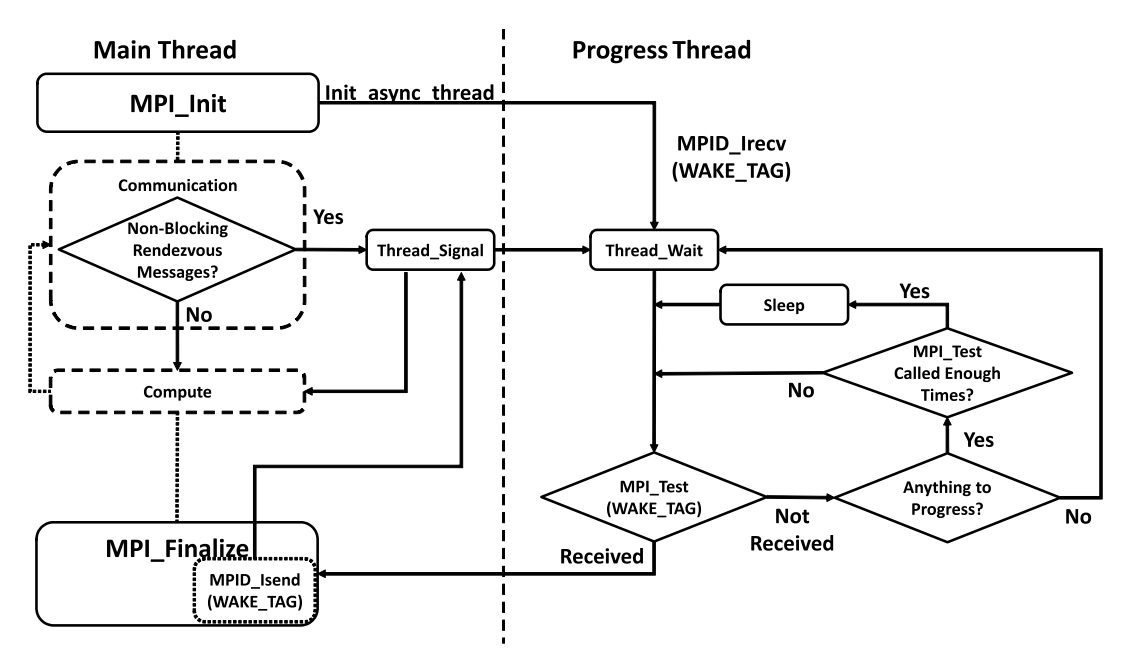
\includegraphics[width=0.8\linewidth]{TexFiles/Figures/Dummy-Diagram.png}
	\caption{Dummy Diagram, adapted from a dummy reference \cite{Li2020}}
	\label{fig:Dummy-Figure}
\end{figure}

\section{A section related to background}
\label{sec-bg-programming-models}

\lipsum[2-4]

\section{A more detailed subsection related to background}

\lipsum[5-6]

Let's have two figures, side by side in Figure \ref{fig:Side-by-Side-Figure}.
You can figure subfigures by \ref{fig:left-sub-figure} and \ref{fig:right-sub-figure}.

\begin{figure}
	\centering
	\begin{subfigure}[b]{0.45\linewidth}
		\centering
		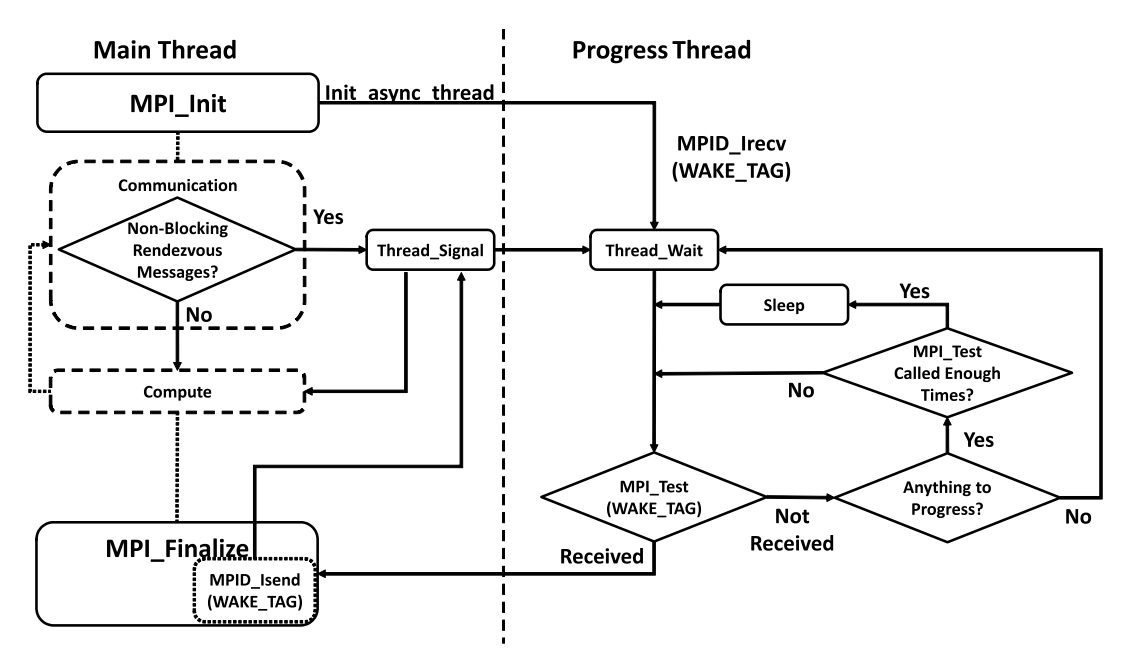
\includegraphics[width=\linewidth]{TexFiles/Figures/Dummy-Diagram.png}
		\caption{Same diagram as before!}
		\label{fig:left-sub-figure}
	\end{subfigure}
	\begin{subfigure}[b]{0.45\linewidth}
		\centering
		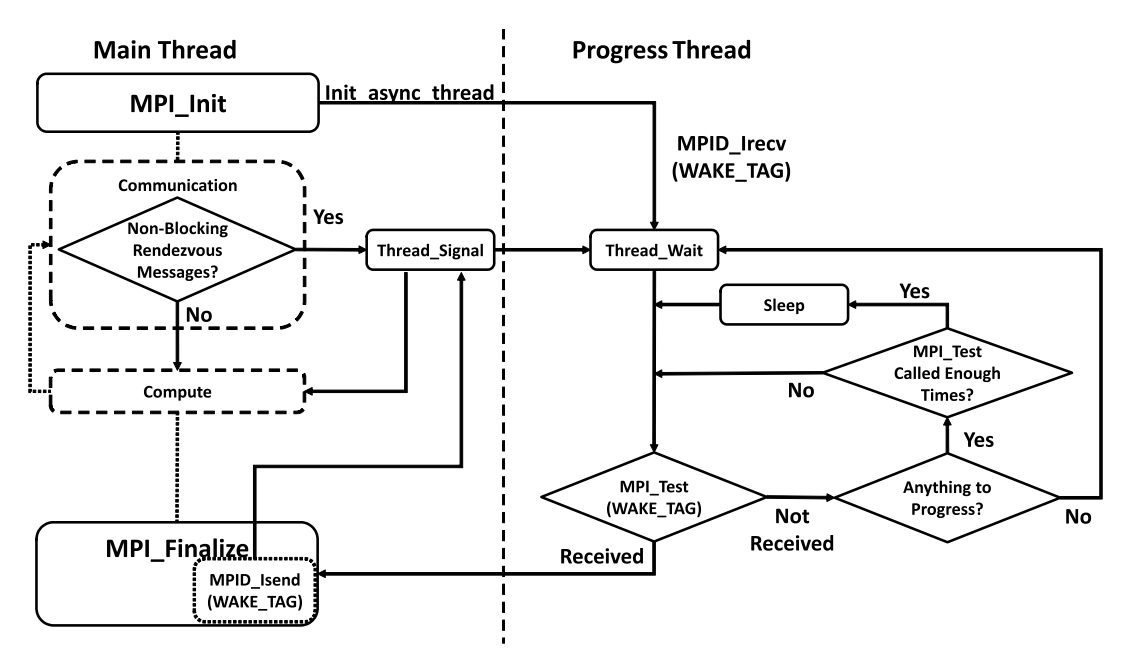
\includegraphics[width=\linewidth]{TexFiles/Figures/Dummy-Diagram.png}
		\caption{Same diagram as before, again!}
		\label{fig:right-sub-figure}
	\end{subfigure}
	\caption{Let's have the Same diagram as before, side by side!}
	\label{fig:Side-by-Side-Figure}
\end{figure}

\textbf{Important thing:} \lipsum[7-7]